% Paquets généraux
\documentclass[a4paper,12pt,titlepage]{article}
\usepackage[T1]{fontenc}
\usepackage[utf8]{inputenc}
\usepackage[french]{babel}
\usepackage[gen]{eurosym}
%\usepackage[dvips]{graphicx}
\usepackage{fancyhdr}
\usepackage{pdfpages} 
\usepackage{multido}
\usepackage{hyperref}
%\usepackage{textcomp}
%\usepackage{aeguill}
\usepackage{schemabloc}
\usepackage[bitstream-charter]{mathdesign}
\usepackage{pstricks}
\usepackage{helvet}

\newcommand{\id}{71}
\newcommand{\nom}{Théorie des mécanismes}
\newcommand{\sequence}{04}
\newcommand{\nomsequence}{Liaisons entre les solides}
\newcommand{\num}{02}
\newcommand{\type}{KH}
\newcommand{\descrip}{Liaisons équivalentes, hyperstatisme, liaisons en série et en parallèle, théorie des graphes}
\newcommand{\competences}{B2-12: Proposer une modélisation des liaisons avec leurs caractéristiques géométriques. \\ &  B2-13: Proposer un modèle cinématique paramétré à partir d'un système réel, d'une maquette numérique ou d'u \\ &  B2-17: Simplifier un modèle de mécanisme. \\ &  B2-18: Modifier un modèle pour le rendre isostatique. \\ &  C1-04: Proposer une démarche permettant d'obtenir une loi entrée-sortie géométrique.  \\ &  C2-05: Caractériser le mouvement d'un repère par rapport à un autre repère. \\ &  C2-06: Déterminer les relations entre les grandeurs géométriques ou cinématiques. }
\newcommand{\nbcomp}{7}
\newcommand{\systemes}{}
\newcommand{\systemesnum}{}
\newcommand{\systemessansaccent}{}
\newcommand{\ilot}{2}
\newcommand{\ilotstr}{02}
\newcommand{\dossierilot}{\detokenize{Ilot_02 }}


\newcommand{\auteurun}{Renaud Costadoat}
\newcommand{\institute}{Lycée Dorian}


\usepackage{color}
\usepackage{xcolor}
\usepackage{colortbl}
\usepackage{helvet}
\renewcommand{\familydefault}{\sfdefault}
\usepackage{amsfonts}
\usepackage{amsmath}
%\usepackage{xspace}
\usepackage{varioref}
\usepackage{tabularx}
%\usepackage{floatflt}
\usepackage{graphics}
\usepackage{wrapfig}
\usepackage{textcomp}
\usepackage{tikz}
\usepackage{wrapfig}
\usepackage{gensymb}
\usepackage[european]{circuitikz}
\usetikzlibrary{babel}
\usepackage{ifthen}
\usepackage{cancel}
\usepackage{etoolbox}
\usepackage{multirow}
%\usepackage{boxedminipage}
\definecolor{gris25}{gray}{0.75}
\definecolor{bleu}{RGB}{18,33,98}
\definecolor{bleuf}{RGB}{42,94,171}
\definecolor{bleuc}{RGB}{231,239,247}
\definecolor{rougef}{RGB}{185,18,27}
\definecolor{rougec}{RGB}{255,188,204}%255,230,231
\definecolor{vertf}{RGB}{103,126,82}
\definecolor{vertc}{RGB}{220,255,191}
\definecolor{forestgreen}{rgb}{0.13,0.54,0.13}
\definecolor{blcr}{rgb}{0.59,0.69,0.84}
\definecolor{blfr}{rgb}{0.32,0.51,0.75}
\definecolor{orfr}{rgb}{0.90,0.42,0.15}
\definecolor{orcr}{rgb}{0.90,0.65,0.50}
\definecolor{orangef}{rgb}{0.659,0.269,0.072}
\definecolor{orange}{rgb}{0.58,0.35,0.063}
\definecolor{orangec}{rgb}{0.43,0.32,0.25}
\definecolor{rcorrect}{rgb}{0.6,0,0}
\definecolor{sequence}{rgb}{0.75,0.75,0.75}
\definecolor{competences}{rgb}{0.61,0.73,0.35}
\definecolor{grisf}{HTML}{222222}
\definecolor{grisc}{HTML}{636363}
\definecolor{normal}{HTML}{4087c4}
\definecolor{info}{HTML}{5bc0de}
\definecolor{success}{RGB}{92,184,92}
\definecolor{warning}{RGB}{240,173,78}
\definecolor{danger}{RGB}{217,83,79}
\hypersetup{                    % parametrage des hyperliens
    colorlinks=true,                % colorise les liens
    breaklinks=true,                % permet les retours à la ligne pour les liens trop longs
    urlcolor= blfr,                 % couleur des hyperliens
    linkcolor= orange,                % couleur des liens internes aux documents (index, figures, tableaux, equations,...)
    citecolor= forestgreen                % couleur des liens vers les references bibliographiques
    }

% Mise en page
\pagestyle{fancy}

\setlength{\hoffset}{-18pt}

\setlength{\oddsidemargin}{0pt} 	% Marge gauche sur pages impaire2s
\setlength{\evensidemargin}{0pt} 	% Marge gauche sur pages paires
\setlength{\marginparwidth}{00pt} 	% Largeur de note dans la marge
\setlength{\headwidth}{481pt} 	 	% Largeur de la zone de tête (17cm)
\setlength{\textwidth}{481pt} 	 	% Largeu\textbf{r de la zone de texte (17cm)
\setlength{\voffset}{-18pt} 		% Bon pour DOS
\setlength{\marginparsep}{7pt}	 	% Séparation de la marge
\setlength{\topmargin}{-30pt} 		% Pas de marge en haut
\setlength{\headheight}{55pt} 		% Haut de page
\setlength{\headsep}{20pt} 		% Entre le haut de page et le texte
\setlength{\footskip}{30pt} 		% Bas de\textbf{ page + séparation
\setlength{\textheight}{700pt} 		% Hauteur de l'icone zone de texte (25cm)
\setlength\fboxrule{1 pt}
\renewcommand{\baselinestretch}{1}
\setcounter{tocdepth}{1}
\newcommand{\cadre}[2]
{\fbox{
  \begin{minipage}{#1\linewidth}
   \begin{center}
    #2\\
   \end{center}
  \end{minipage}
 }
}


\newcommand{\titre}[1]
{\begin{center}
\cadre{0.8}{\huge #1} 
\end{center}
}

\newcounter{num_quest} \setcounter{num_quest}{0}
\newcounter{num_rep} \setcounter{num_rep}{0}

\newcommand{\question}[1]{\refstepcounter{num_quest}\par
~\ \\ \textbf{Question \arabic{num_quest} : }#1\label{q\the\value{num_quest}}\par
}

\newcommand{\reponse}[1]
{\noindent
\rule{\linewidth}{.5pt}\\
\textbf{Question \refstepcounter{num_rep}\ref{q\the\value{num_rep}} :} ~\ \\
#1}

% En tête et pied de page
\lhead{\nom}
\rhead{
\includegraphics[width=2cm]{../../img/logo}}
\lfoot{Renaud Costadoat}
\cfoot{Page \thepage}

\fancypagestyle{correction}{%
  \fancyhf{}
  \lhead{\colorbox{danger}{\begin{minipage}{0.65\paperwidth} \textcolor{white}{\textbf{Correction}} \end{minipage}} }
  \rhead{
\includegraphics[width=2cm]{../../img/logo}}
  \lfoot{Renaud Costadoat}
  \rfoot{\colorbox{danger}{\begin{minipage}{0.6\paperwidth} \begin{flushright}\textcolor{white}{\textbf{Correction}}\end{flushright} \end{minipage}} }}

\renewcommand{\footrulewidth}{0.4pt}

\usepackage{eso-pic}
\newcommand{\BackgroundPic}{%
\put(0,0){%
\parbox[b][\paperheight]{\paperwidth}{%
\vfill
\begin{center}
\hspace{0.5cm}\vspace{0.5cm}

\includegraphics[width=\paperwidth,height=\paperheight,%
keepaspectratio]{../../img/fond3}%
\end{center}
\vfill
}}}

\newcommand{\BackgroundPicdeux}{%
\put(25,-30){%
\parbox[b][\paperheight]{\paperwidth}{%
\vfill
\begin{center}
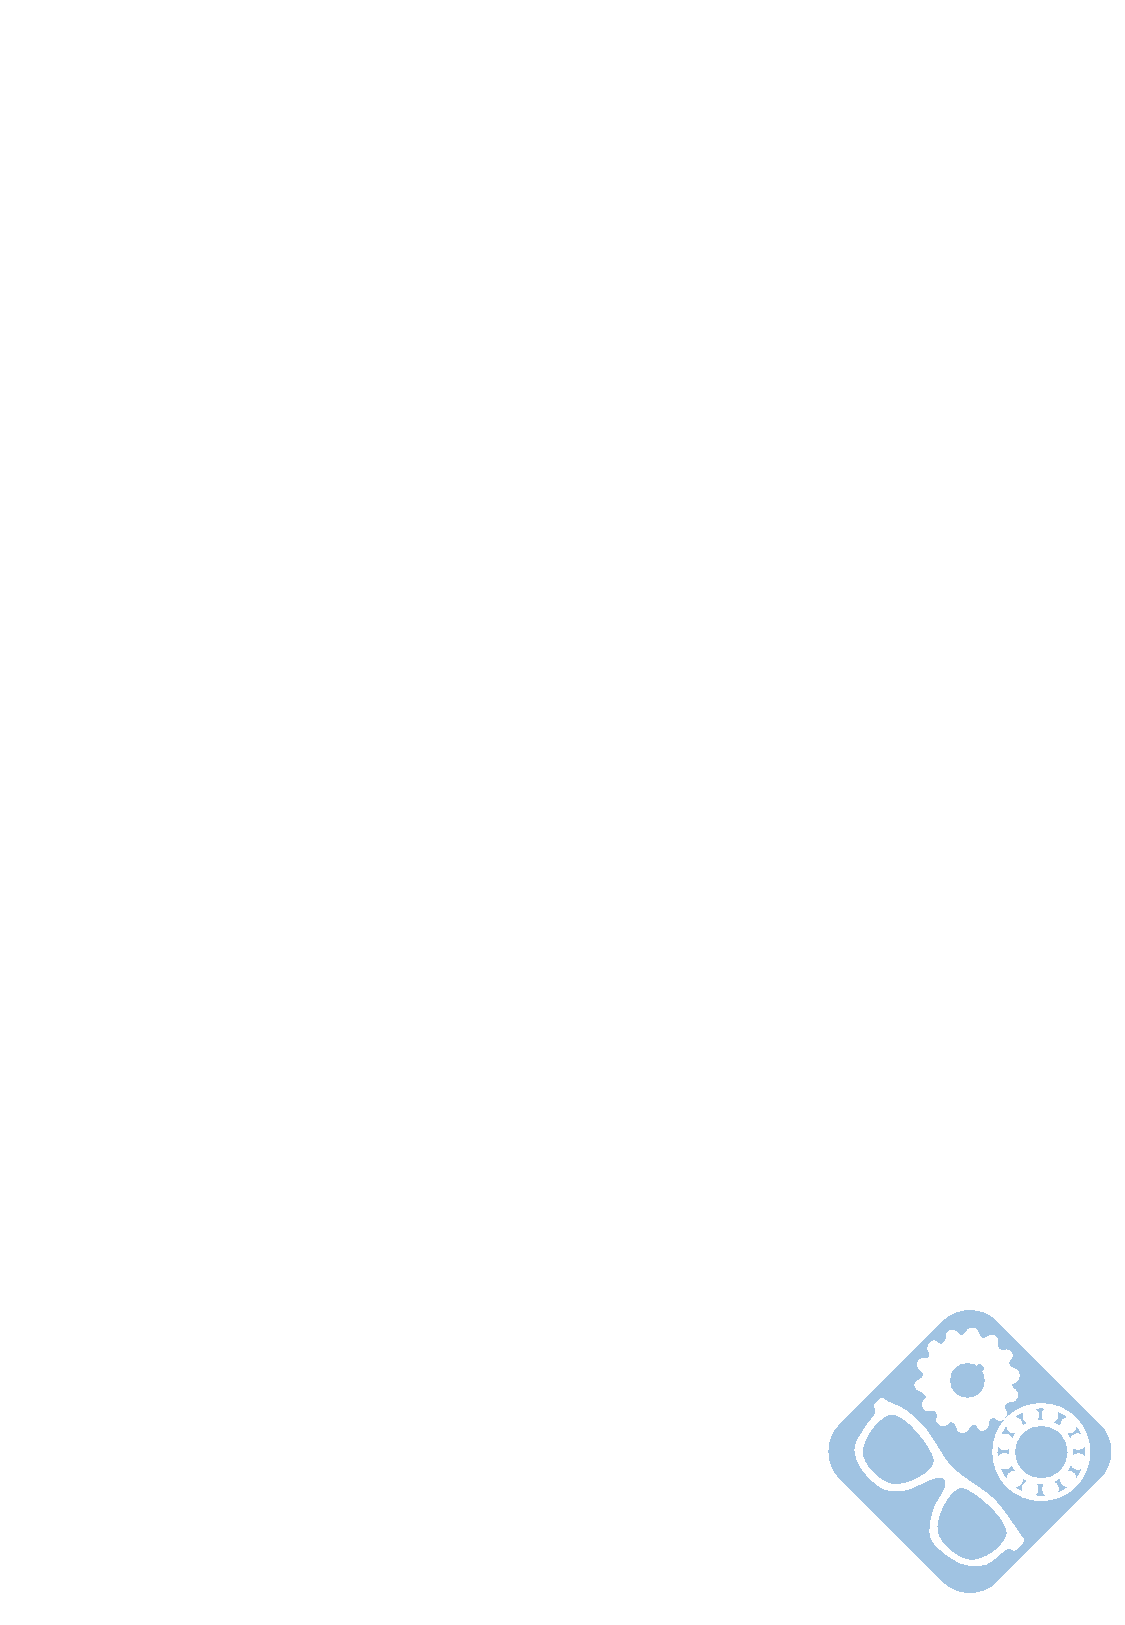
\includegraphics[width=\paperwidth,height=\paperheight,%
keepaspectratio]{../../img/fond4}%
\end{center}
\vfill
}}}

\begin{document}

\AddToShipoutPicture{\BackgroundPicdeux}

\pagestyle{fancy}

\section{Planeur sous-marin}

\subsection{Présentation}

\begin{figure}[!h]
 \begin{minipage}{0.6\linewidth}
L'environnement marin est un système complexe caractérisé par d'importantes interactions entre des processus physiques, chimiques et biologiques. La forte variabilité de ces processus et de leurs interactions rend difficile toute étude de l'écosystème marin, d'une part parce qu'il est nécessaire de mesurer les paramètres physiques, chimiques et biologiques simultanément, et d'autre part parce que ces mesures doivent être faites avec des résolutions spatiale et temporelle suffisantes.
 \end{minipage}
 \hfill
  \begin{minipage}{0.35\linewidth}
   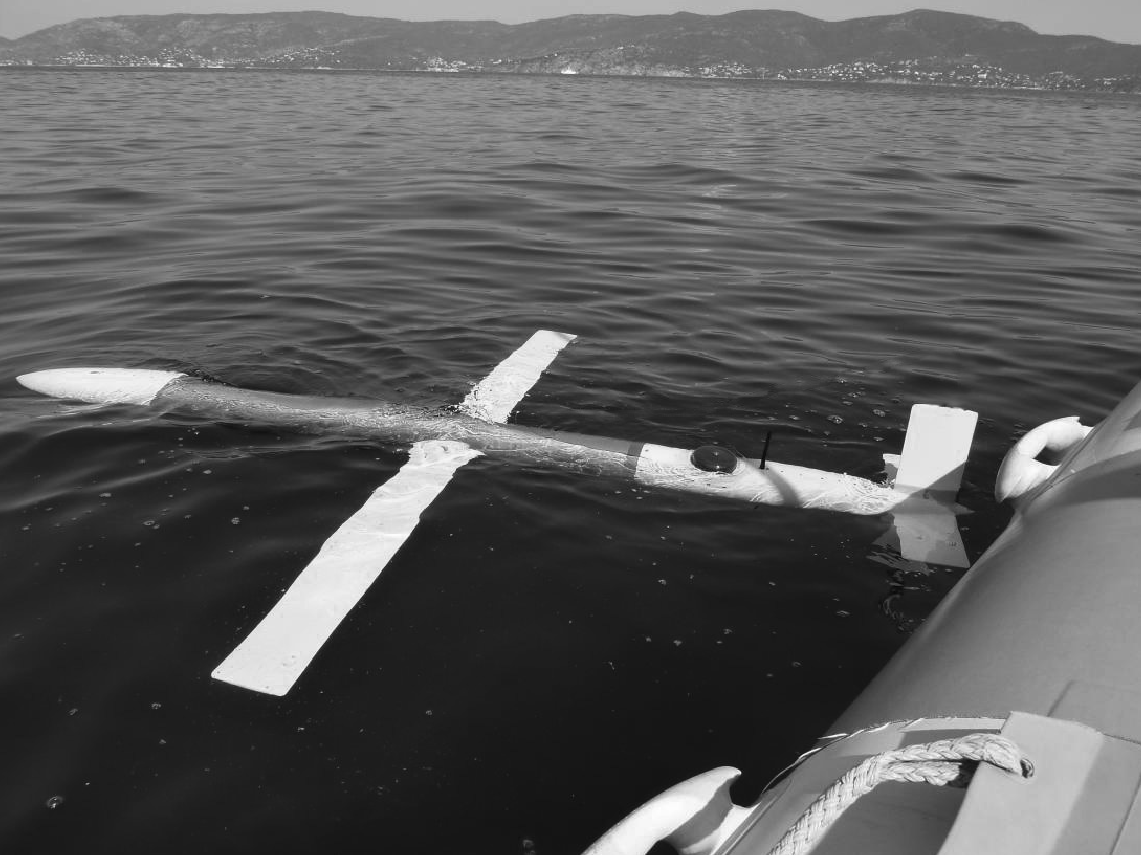
\includegraphics[width=0.9\linewidth]{img/planeur.png}
  \end{minipage}
\end{figure}

\subsection{Analyse de l'équilibre en déplacement}

En mouvement, l'aile génère une portance dont l'inclinaison par rapport à l'horizontale permet la propulsion du planeur.

Nous allons réaliser le bilan des actions extérieures au planeur en phase de montée et déterminer l'action de propulsion en fonction de la poussée d'Archimède ainsi que le besoin en précision du vérin.

Nous supposons que l'équilibre statique est vérifié (termes dynamiques négligés).

A l'échelle de l'esquisse, la différence entre la poussée d'Archimède, d'intensité notée $A$, et le poids d'intensité $P$ est: $A-P=10N$, ($A>P$ en montée, force de portance suivant $-\overrightarrow{y_1}$). La masse du sous-marin est de 50kg et la distance AC' vaut 200mm.

\paragraph{Question 1 :} Réaliser le tracé de la force hydrodynamique $\overrightarrow{F_H}$, puis de ces composantes de portance $F_p$, support $(A,\overrightarrow{y_1})$ et de traînée $F_t$ support $(C',\overrightarrow{x_1})$. En déduire les expressions analytiques de $F_p$ et $F_t$ en fonction de $A$, $P$ et des caractéristiques de fonctionnement.

\begin{center}
\centering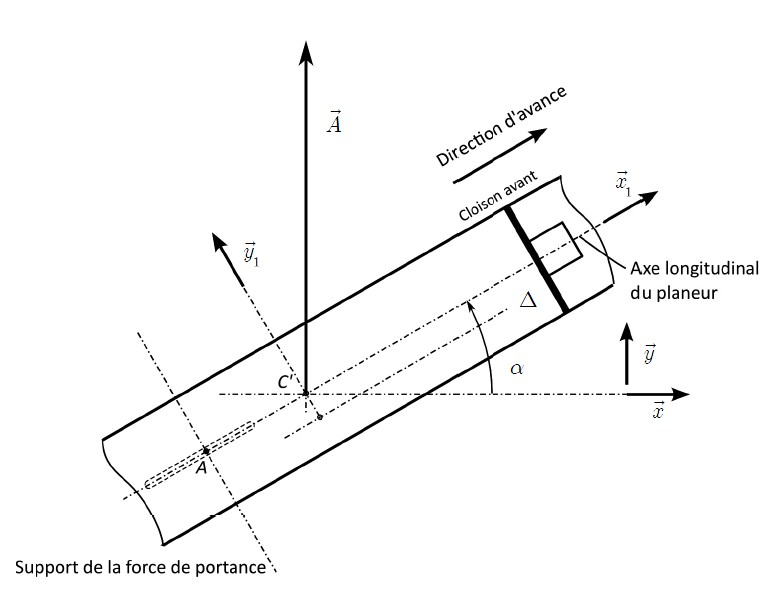
\includegraphics[width=0.7\linewidth]{img/plan_Q1.jpg}
\end{center}

\paragraph{Question 2:} Le centre de gravité G' du planeur est situé sur l'axe $\Delta=(G_0,\overrightarrow{x_1})$. Déterminer sa position et tracer le poids sur l'esquisse. Vous préciserez le théorème utilisé pour déterminer sa position.

\begin{center}
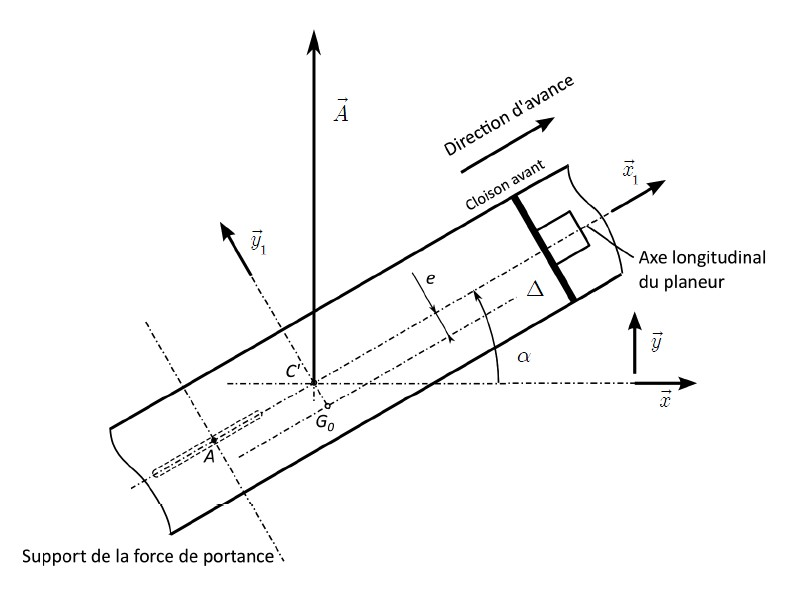
\includegraphics[width=0.7\linewidth]{img/plan_Q2.jpg}
\end{center}

\begin{minipage}{0.58\linewidth}
\paragraph{Question 3:} Déterminer la relation entre l'angle de tangage $\alpha$ du planeur en mouvement et le déplacement $\delta$ de son centre de gravité.

En déduire le déplacement du piston nécessaire pour obtenir un angle de tangage de 30\textdegree. Le résultat est-il celui de la courbe ? 

\paragraph{Question 4:} Estimer la précision nécessaire sur le déplacement du piston pour obtenir, autour de 30\textdegree, un contrôle de l'angle de tangage répondant au cahier des charges (marge de 15\%). Conclure.
\end{minipage}
\hfill
\begin{minipage}{0.4\linewidth}
\centering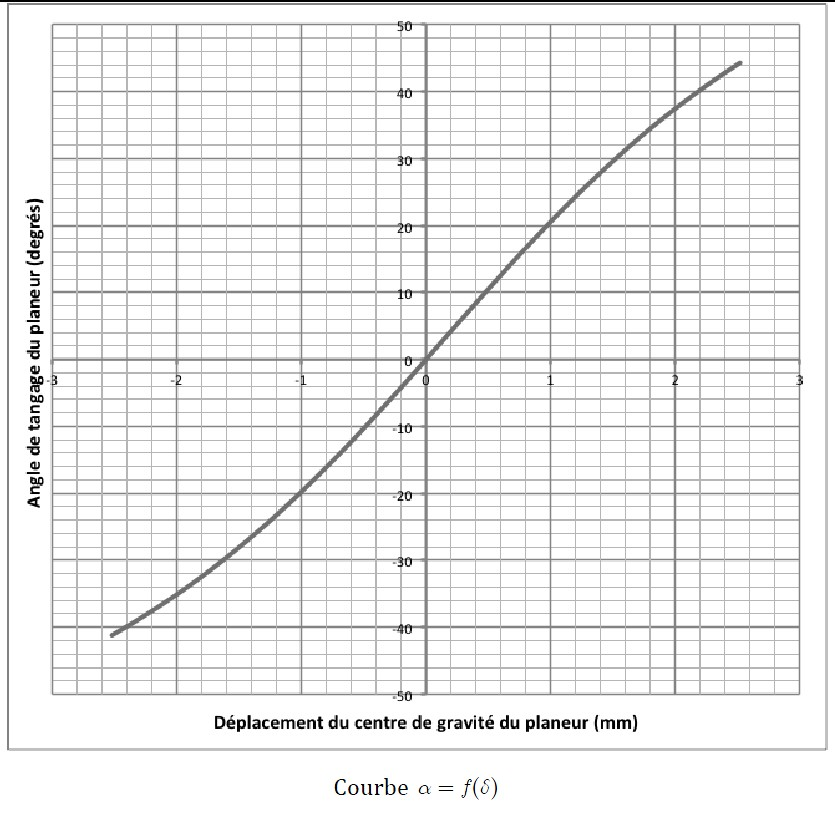
\includegraphics[width=0.9\linewidth]{img/plan_Q3.jpg}
\end{minipage}

\begin{minipage}{0.38\linewidth}
{\centering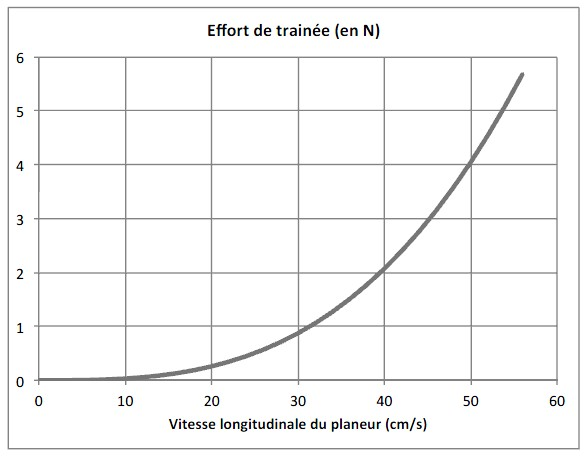
\includegraphics[width=0.9\linewidth]{img/plan_Q5.jpg}}
\end{minipage}
\hfill
\begin{minipage}{0.6\linewidth}
La section du piston est de $5 000 mm^2$.

\paragraph{Question 5:} En déduire, pour cet angle de 30\textdegree, l'intensité de $\overrightarrow{F_H}$ et la composante de traînée $F_t$. Tracer le point de fonctionnement sur le graphique du cahier réponses. En déduire la vitesse longitudinale du planeur.
\end{minipage}

\newpage

\section{Micromanipulateur}

\begin{minipage}{0.6\linewidth}
Le micromanipulateur doit déplacer un échantillon de un kilogramme. L'objecif de cette partie est de définir l'effort que devront fournir les moteurs pour maintenir l'échantillon dans une position mais aussi pour le déplacer.

Données:
\begin{itemize}
 \item les frottements secs sont négligeables,
 \item pas de la vis à bille: $p_v=10^{-3}m$,
\end{itemize}
\end{minipage}
\hfill
\begin{minipage}{0.37\linewidth}
\centering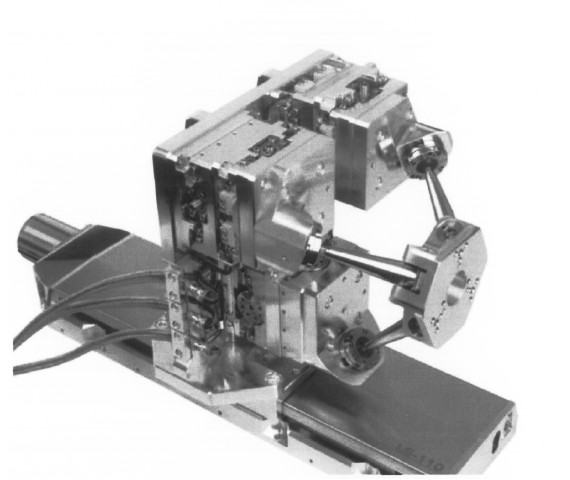
\includegraphics[width=0.9\linewidth]{img/Micro.jpg}
\end{minipage}

~\

Les moteurs pas àpas ne comportant pas de frein, le couple nécessaire au maintien en position de la plateforme est obtenu par application d'une tension dans les bobines du moteur. Il faut déterminer ce couple pour l'intégrer dans la commande des moteurs.

~\

Hypothèses:
\begin{itemize}
 \item le système est, à tout point de vue, symétrique par rapport au plan $O_0,\overrightarrow{x_0},\overrightarrow{z_0}$,
 \item le système est dans la position de référence,
 \item les liaisons sont sans frottement,
 \item l'étude spatiale peut être ramenée, par projection, à deux études dans les deux plans $O_0,\overrightarrow{x_0},\overrightarrow{z_0}$ et $O_0,\overrightarrow{x_0},\overrightarrow{y_0}$,
 \item le système étant en équilibre, la projection du système de forces dans deux plans orthogonaux permet d'utiliser les méthodes de la statique graphique successivement dans chacun de ces plans.
\end{itemize}

\begin{center}
\centering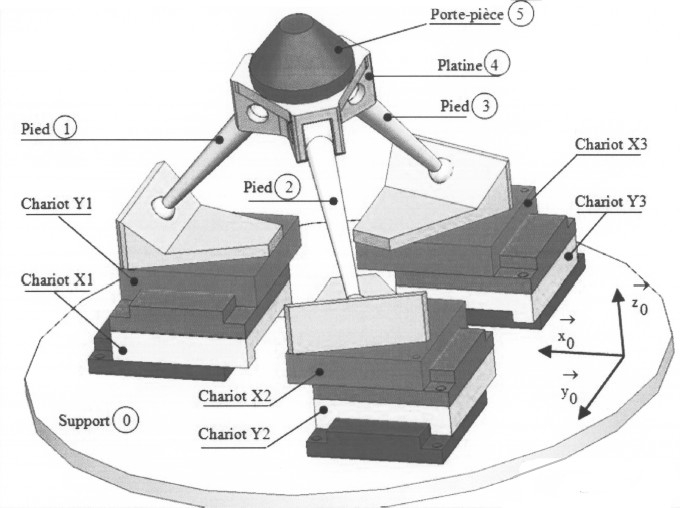
\includegraphics[width=0.8\linewidth]{img/Micro2.jpg}
\end{center}

\paragraph{Question 1:} Sur le document réponse, à partir du poid tracé en $G_{\Sigma}$ sur $O_0,\overrightarrow{z_0}$, déterminer graphiquement l'action mécanique dans la liaison sphérique en $A_1$.

\paragraph{Question 2:} Soit $\overrightarrow{F_{1 \rightarrow X_1}}.\overrightarrow{x_0}=F$, déterminer en fonction de F, l'expression du couple $C_s$ que le moteur du charriot $X_1$ doit exercer pour que le système reste en équilibre.

\begin{center}
\centering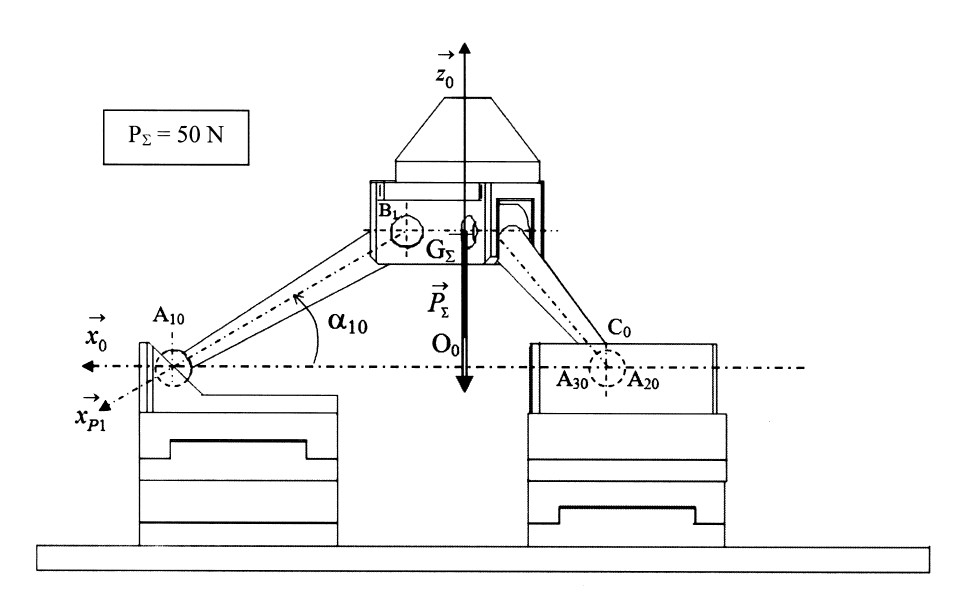
\includegraphics[width=0.9\linewidth]{img/Micro_DR.jpg}
\end{center}

\newpage

\section{Doseur de granules plastiques}

\begin{minipage}{0.6\linewidth}
L'injection de matière plastique est une technique qui consiste à pousser de la matière plastique chauffée dans un moule afin de réaliser une pièce. La machine qui réalise cette opération est appelée \og presse à injecter \fg.
\end{minipage}
\hfill
\begin{minipage}{0.37\linewidth}
\centering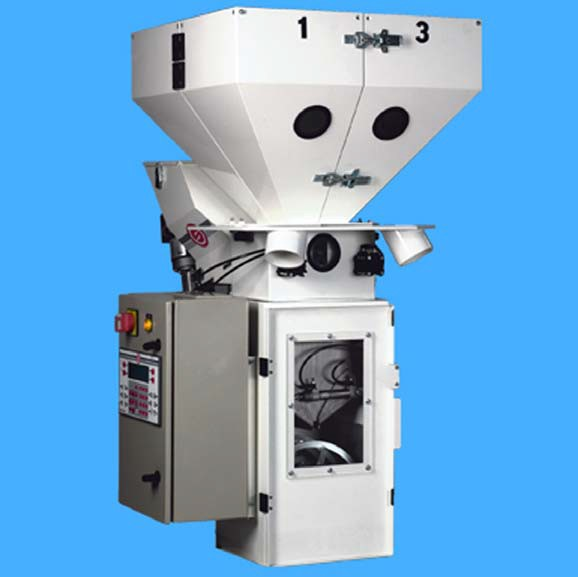
\includegraphics[width=0.8\linewidth]{img/doseur1.jpg}
\end{minipage}

\textbf{Première modélisation du capteur}

Remarque : dans le texte suivant \og trémie \fg désigne la trémie de pesée et les granulés qu'elle contient. L'objectif est de mesurer le poids de la trémie de pesage, soit la résultante P du torseur :

$\left\{\tau_{pesanteur \rightarrow tremie}\right\}=\left\{
\begin{array}{c}
-P.\overrightarrow{y} \\
0.\overrightarrow{z}
\end{array}\right\}_G$

G étant le centre de gravité de la tremie.

\begin{minipage}{0.6\linewidth}
Un capteur supporte la trémie. Un de ses cotés est lié au bati de la machine, son autre coté étant accroché en un point K à la trémie.
Lors de la chute des granulés, le centre de gravité de la masse des granulés occupe une position variable et inconnue.
\end{minipage}
\hfill
\begin{minipage}{0.37\linewidth}
\centering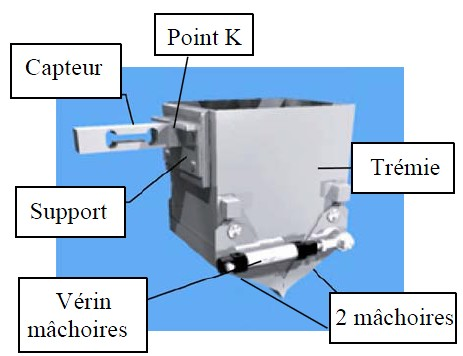
\includegraphics[width=0.8\linewidth]{img/doseur4.jpg}
\end{minipage}

Le torseur des actions mécaniques exercées par la trémie sur le capteur peut s'écrire:

$\left\{\tau_{pesanteur \rightarrow capteur}\right\}=\left\{
\begin{array}{c}
-P.\overrightarrow{y} \\
M_K.\overrightarrow{z}
\end{array}\right\}_K$

\begin{minipage}{0.6\linewidth}
Le capteur réel peut être modélisé par une structure parallèlogramme 4 barres liées par 4 liaisons pivots élastiques.

Pour que la mesure donnée par le capteur soit indépendante de la position de G, le comportement du capteur ne doit pas dépendre du moment $M_K$.
\end{minipage}
\hfill
\begin{minipage}{0.37\linewidth}
\centering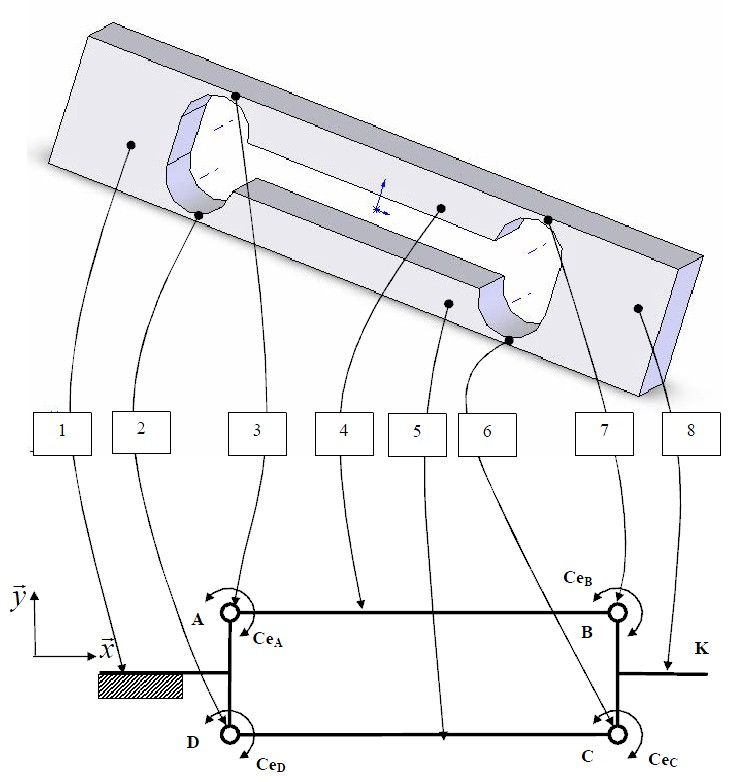
\includegraphics[width=0.8\linewidth]{img/doseur2.jpg}
\end{minipage}

Pour cela on va étudier dans un premier temps un modèle simplifié dans lequel seule la liaison pivot en A est une liaison pivot élastique, les autres liaisons pivot en B, C, D étant parfaites.

\begin{center}
\centering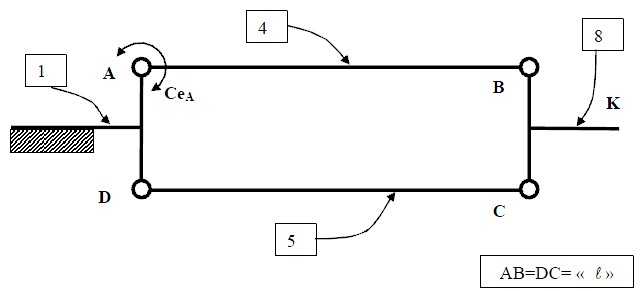
\includegraphics[width=0.8\linewidth]{img/doseur3.jpg}
\end{center}

La technologie du capteur permet de mesurer $C_{eA}$. On souhaite donc vérifier qu'il existe une relation $P=f(C_{eA})$ indépendante de $M_K$.

\paragraph{Question 1:} Trouver la relation $P=f(C_{eA})$ par statique graphique. Pour cela:

\begin{itemize}
 \item Isoler 5, si possible déterminer $C_X$, $C_Y$, $D_X$ ou $D_Y$, justifier la réponse.

$\left\{\tau_{8 \rightarrow 5}\right\}=\left\{
\begin{array}{c}
C_X.\overrightarrow{x}+C_Y.\overrightarrow{y} \\
0.\overrightarrow{z}
\end{array}\right\}_C$ et $\left\{\tau_{1 \rightarrow 5}\right\}=\left\{
\begin{array}{c}
D_X.\overrightarrow{x}+D_Y.\overrightarrow{y} \\
0.\overrightarrow{z}
\end{array}\right\}_D$

Justifier la réponse.
 \item Isoler 8 et en déduire en fonction de $P$ la composante $B_Y$ du torseur

$\left\{\tau_{4 \rightarrow 8}\right\}=\left\{
\begin{array}{c}
-B_X.\overrightarrow{x}-B_Y.\overrightarrow{y} \\
0.\overrightarrow{z}
\end{array}\right\}_B$

Préciser l'équation utilisée. Reporter la valeur de $B_Y$ sur le document réponse,

 \item Isoler 4 et en déduire en fonction de $P$ la composante $C_{eA}$ du torseur 

$\left\{\tau_{1 \rightarrow 4}\right\}=\left\{
\begin{array}{c}
A_X.\overrightarrow{x}+A_Y.\overrightarrow{y} \\
C_{eA}.\overrightarrow{z}
\end{array}\right\}_A$

Préciser l'équation utilisée. Reporter la valeur de $C_{eA}$ sur le document réponse.
\end{itemize}

%
%\textbf{Deuxième modélisation du capteur}
%
%Le capteur d'efforts utilisé est en réalité constitué de 4 zones rigides 1, 8, 4 et 5 reliées par 4 zones déformables 2, 3, 6 et 7 que l'on peut modéliser par quatre liaisons pivots élastiques. On retient un modèle d'étude plan et les torseurs d'efforts transmissibles dans chacune des liaisons pivots non parfaites peuvent s'écrire :
%
%\begin{itemize}
% \item Pour la liaison 3: $\left\{\tau_{1 \rightarrow 4}\right\}=\left\{
%\begin{array}{c}
%A_X.\overrightarrow{x}+A_Y.\overrightarrow{y} \\
%C_{eA}.\overrightarrow{z}
%\end{array}\right\}_A$,
%
% \item Pour la liaison 7 :
%$\left\{\tau_{8 \rightarrow 4}\right\}=\left\{
%\begin{array}{c}
%B_X.\overrightarrow{x}+B_Y.\overrightarrow{y} \\
%C_{eB}.\overrightarrow{z}
%\end{array}\right\}_B$
%
% \item Pour la liaison 6 :
%$\left\{\tau_{8 \rightarrow 5}\right\}=\left\{
%\begin{array}{c}
%C_X.\overrightarrow{x}+C_Y.\overrightarrow{y} \\
%C_{eC}.\overrightarrow{z}
%\end{array}\right\}_C$
%
% \item Pour la liaison 2 :
%$\left\{\tau_{1 \rightarrow 5}\right\}=\left\{
%\begin{array}{c}
%D_X.\overrightarrow{x}+D_Y.\overrightarrow{y} \\
%C_{eD}.\overrightarrow{z}
%\end{array}\right\}_D$
%\end{itemize}
%
%L'action de la trémie sur le capteur est modélisée par le torseur :

\ifdef{\public}{\end{document}}{}

\newpage

\pagestyle{correction}\setcounter{section}{0}

\paragraph{Question 1:}

\begin{center}
	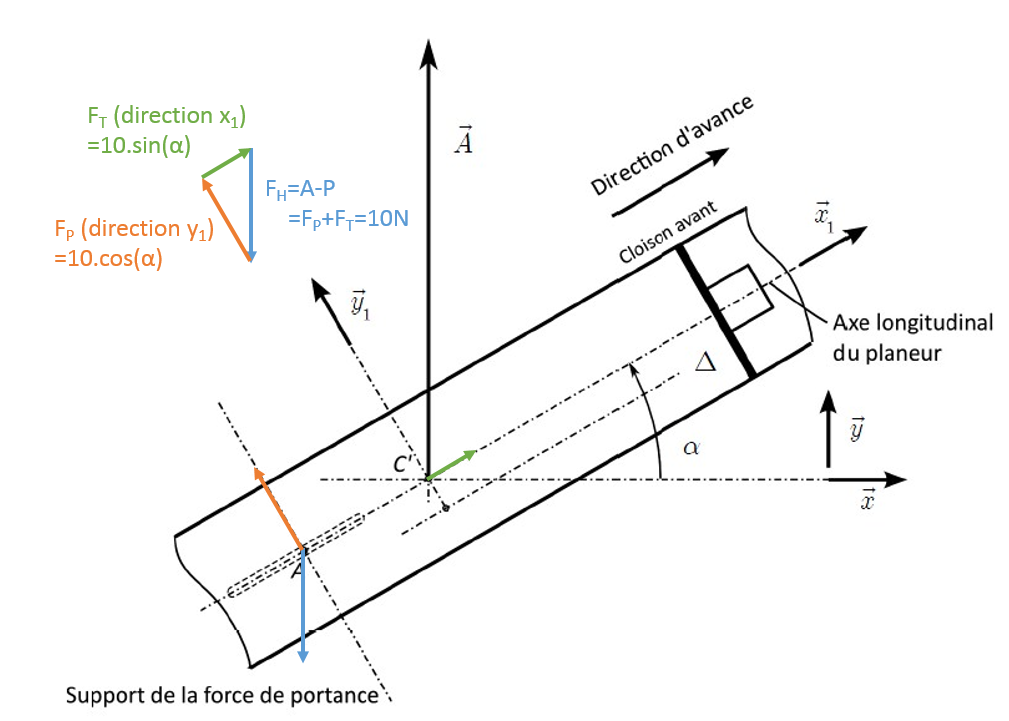
\includegraphics[width=0.8\linewidth]{img/Cor1}
\end{center}

\paragraph{Question 2:}

\begin{center}
	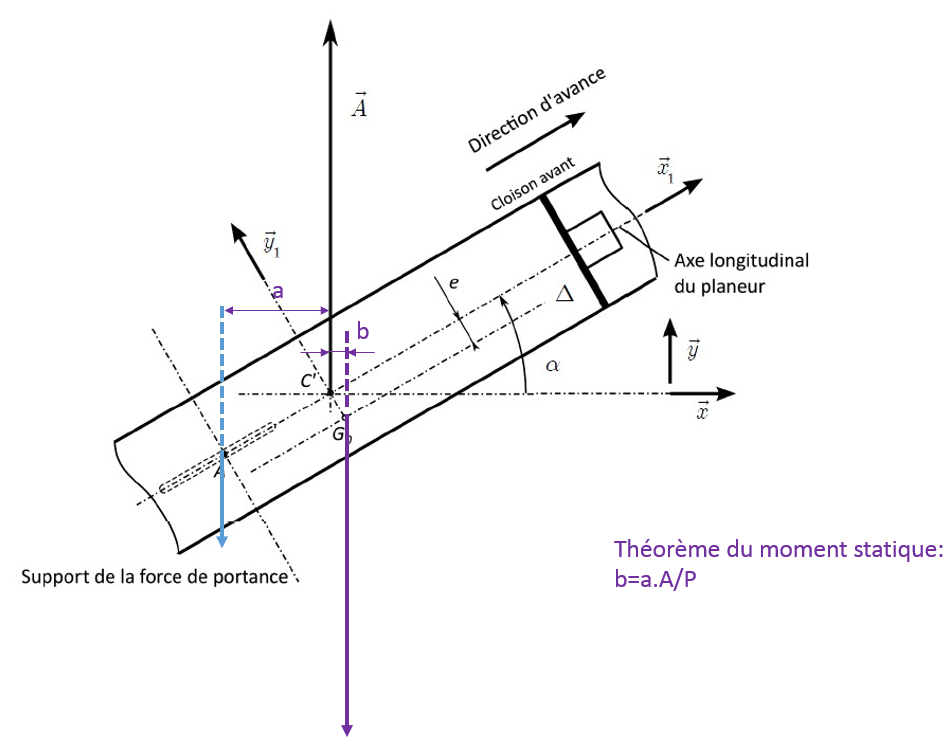
\includegraphics[width=0.8\linewidth]{img/Cor2}
\end{center}

\newpage

\paragraph{Question 3:}

\begin{center}
	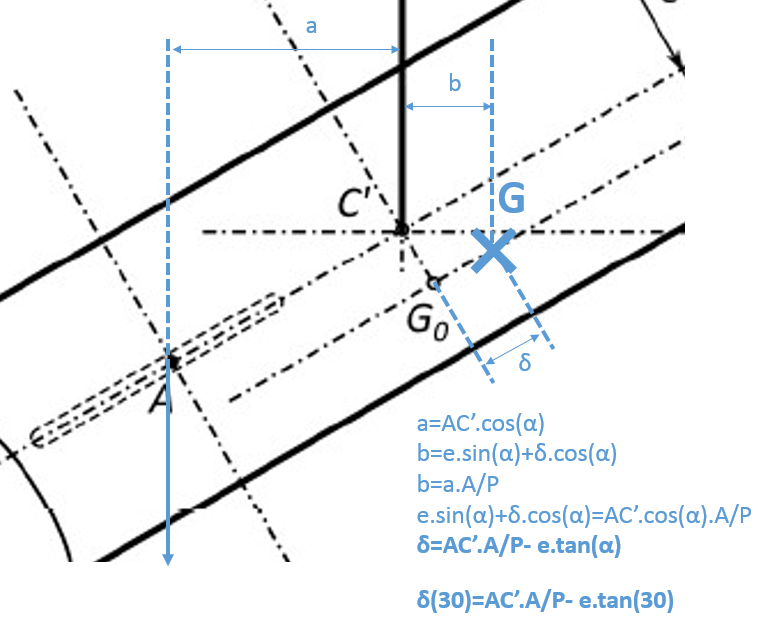
\includegraphics[width=0.8\linewidth]{img/Cor3}
\end{center}

\end{document}